\documentclass[11pt,a4paper]{article}
\usepackage[T1]{fontenc}
\usepackage[utf8]{inputenc}
\usepackage{lmodern}
\usepackage{amsmath}
\usepackage[margin=2.4cm]{geometry}
\usepackage{booktabs}
\usepackage{tabularx}
\usepackage{longtable}
\usepackage{array}
\usepackage{graphicx}
\usepackage{float}
\usepackage[dvipsnames]{xcolor}
\usepackage{enumitem}
\usepackage{titlesec}
\usepackage{parskip}
\usepackage{setspace}
\usepackage{needspace}
\usepackage{tikz}
\usetikzlibrary{positioning,arrows.meta,fit,backgrounds,calc,shapes.geometric}
\usepackage[hidelinks]{hyperref}

\setstretch{1.3}
\setlength{\parskip}{0.9em}
\setlist{itemsep=0.5em, topsep=0.6em}
\renewcommand{\arraystretch}{1.45}
\definecolor{accent}{RGB}{30,80,150}
\titleformat{\section}{\Large\bfseries\color{accent}}{\thesection}{0.8em}{}
\titleformat{\subsection}{\large\bfseries}{\thesubsection}{0.8em}{}
\titlespacing*{\section}{0pt}{2.2em}{1.0em}
\titlespacing*{\subsection}{0pt}{1.6em}{0.7em}
\newcolumntype{L}{>{\raggedright\arraybackslash}X}
\newcolumntype{P}[1]{>{\raggedright\arraybackslash}p{#1}}
\newcommand{\file}[1]{\texttt{\small #1}}
\newcommand{\keybox}[1]{\par\smallskip\noindent\colorbox{accent!8}{\parbox{\dimexpr\linewidth-2\fboxsep}{\vspace{0.5em}#1\vspace{0.5em}}}\par\medskip}
\newcommand{\tablestart}{\Needspace{8\baselineskip}}

% ---- colours of the system diagrams (one per MQTT topic / kind of traffic)
\definecolor{cSensor}{RGB}{37,99,235}     % sensors/<node>
\definecolor{cAlert}{RGB}{220,38,38}      % ids/alerts
\definecolor{cStats}{RGB}{22,163,74}      % ids/stats
\definecolor{cMit}{RGB}{124,58,237}       % ids/mitigation/status
\definecolor{cStatus}{RGB}{100,116,139}   % ids/status
\definecolor{cCmd}{RGB}{234,88,12}        % cmd/mitigation
\definecolor{cAttack}{RGB}{153,27,27}     % attack traffic
\definecolor{cBot}{RGB}{161,98,7}         % bot master commands (UDP, not MQTT)
\definecolor{cPi}{RGB}{220,38,90}
\definecolor{cLap}{RGB}{51,65,85}
\definecolor{cNode}{RGB}{8,145,178}
\newcommand{\topicdot}[1]{\textcolor{#1}{\rule{0.9em}{0.9em}}}

\tikzset{
  box/.style={draw=#1!70!black, fill=#1!8, rounded corners=4pt, align=center, font=\small, line width=0.7pt,
              inner sep=6pt},
  box/.default=gray,
  group/.style={draw=#1, rounded corners=8pt, line width=1.1pt, inner sep=10pt},
  grouplabel/.style={font=\bfseries\small, text=#1, fill=white, inner sep=3pt},
  pub/.style={-{Stealth[length=7pt]}, line width=1.3pt, draw=#1},
  deliver/.style={-{Stealth[length=7pt]}, line width=1.3pt, draw=#1, dashed},
  attack/.style={-{Stealth[length=8pt]}, line width=1.8pt, draw=cAttack, densely dashed},
  botcmd/.style={-{Stealth[length=7pt]}, line width=1.3pt, draw=cBot, densely dotted},
  lbl/.style={font=\scriptsize\ttfamily, text=#1, fill=white, inner sep=1.5pt},
  flow/.style={-{Stealth[length=6pt]}, line width=1pt, draw=gray!70!black},
}

\begin{document}

\begin{titlepage}
\centering
\vspace*{5cm}
{\Huge\bfseries\color{accent} TinyIDS\par}
\vspace{1.2em}
{\LARGE The system and its machine-learning part, explained\par}
\vspace{2.5em}
{\large Design, data, training, model and results of the detector running on the Raspberry Pi\par}
\vfill
{\large 18 November 2026\par}
\vspace{2cm}
\end{titlepage}

\tableofcontents
\newpage

% ---------------------------------------------------------------------------------------------------------------
\section{What the system does, in one page}

TinyIDS is an intrusion detector that runs on a Raspberry Pi~4 (the network gateway of our IoT testbed).

\begin{enumerate}
  \item The Pi captures every packet. Every \textbf{10 packets} from one sender form a \textbf{window}.
  \item For each window it computes \textbf{14 numbers}: packet sizes, TCP flags and protocol shares.
  \item One small \textbf{LightGBM} model reads the 14 numbers and answers one of 3 classes:
        \textbf{Benign} (normal), \textbf{Flood} (DoS / DDoS flood) or \textbf{Recon} (scanning, e.g.\ nmap).
  \item If it says attack, the Pi blocks the sender and the dashboard shows the \textbf{top-3 reasons}
        (SHAP values: which of the 14 numbers pushed the decision most).
  \item Things the model cannot see (DoS vs DDoS, spoofing, MQTT brute force) are handled by simple rules.
\end{enumerate}

\keybox{\textbf{In one sentence:} the model judges \emph{what the traffic looks like} (flood, scan or normal);
rules answer \emph{who and how many}.}

% ---------------------------------------------------------------------------------------------------------------
\newpage
\section{High-level design (HLD)}\label{sec:hld}

\subsection{The machines and what runs on them}

The whole testbed is \textbf{5 devices on one Wi-Fi network}: 3 NodeMCU boards, 1 Raspberry Pi~4 and 1 laptop.
The Pi is the centre: it runs the MQTT broker that everything talks to, and the detector that watches every packet
arriving at it.

\begin{figure}[H]
\centering
\resizebox{\linewidth}{!}{%
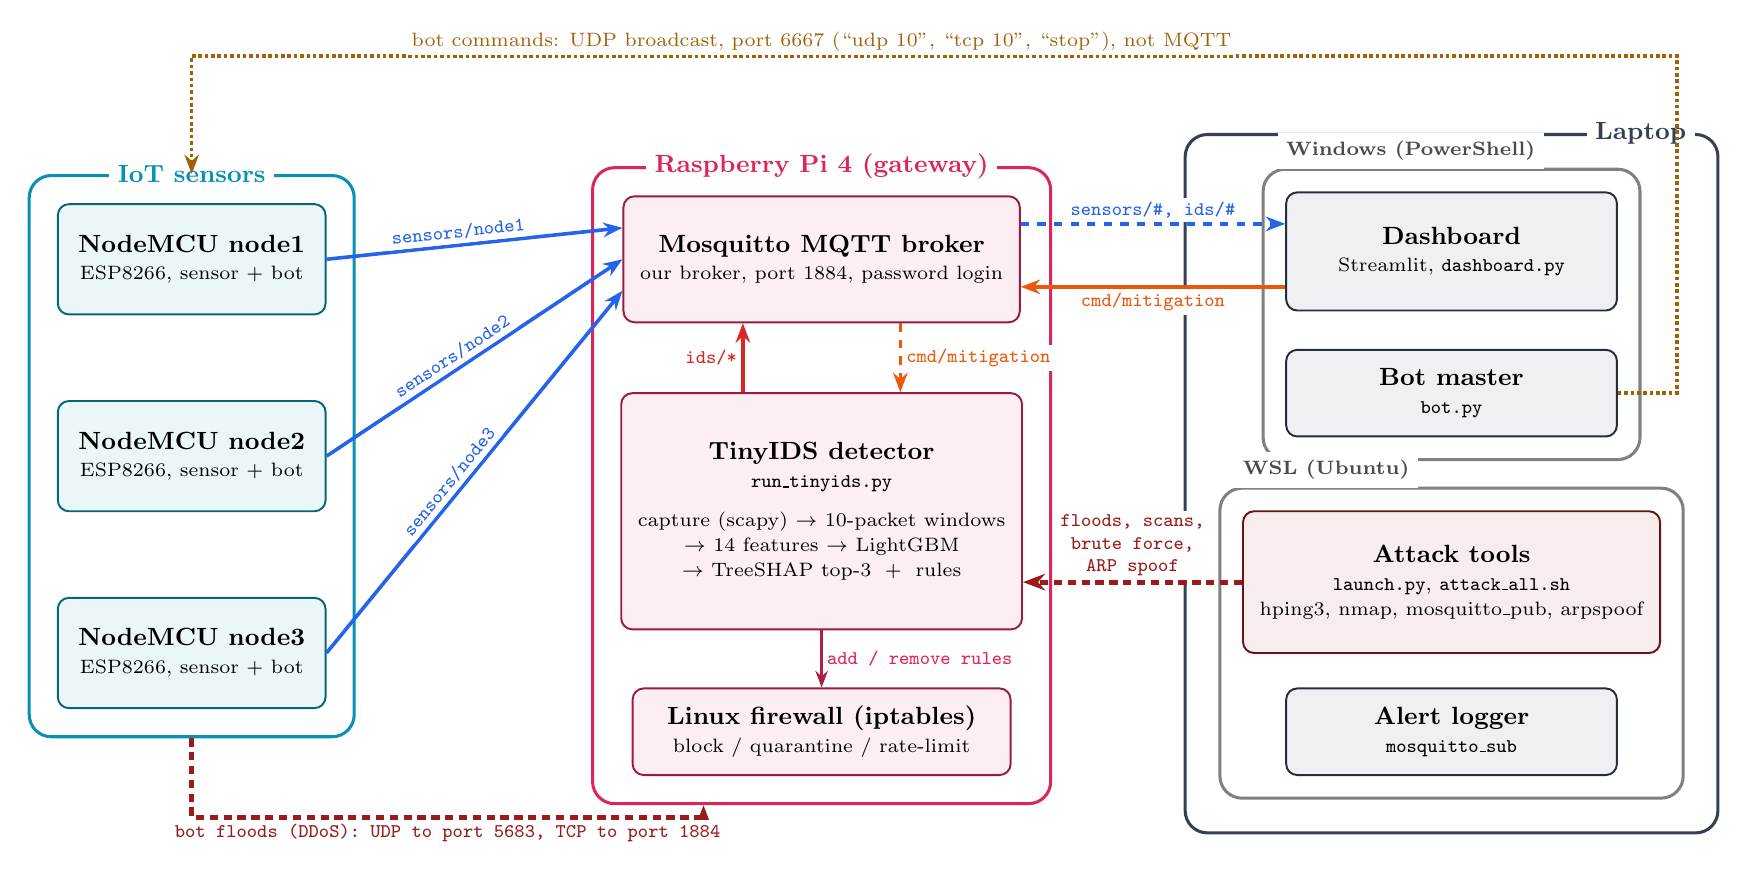
\begin{tikzpicture}[font=\small]

% ---------------- NodeMCUs
\node[box=cNode, minimum width=3.4cm, minimum height=1.4cm] (n1) at (0,3.4)
  {\textbf{NodeMCU node1}\\[-1pt]{\scriptsize ESP8266, sensor + bot}};
\node[box=cNode, minimum width=3.4cm, minimum height=1.4cm] (n2) at (0,0.9)
  {\textbf{NodeMCU node2}\\[-1pt]{\scriptsize ESP8266, sensor + bot}};
\node[box=cNode, minimum width=3.4cm, minimum height=1.4cm] (n3) at (0,-1.6)
  {\textbf{NodeMCU node3}\\[-1pt]{\scriptsize ESP8266, sensor + bot}};
\begin{scope}[on background layer]
  \node[group=cNode, fit=(n1)(n2)(n3)] (gN) {};
\end{scope}
\node[grouplabel=cNode] at (gN.north) {IoT sensors};

% ---------------- Raspberry Pi
\node[box=cPi, minimum width=4.8cm, minimum height=1.6cm] (broker) at (8,3.4)
  {\textbf{Mosquitto MQTT broker}\\[-1pt]{\scriptsize our broker, port 1884, password login}};
\node[box=cPi, minimum width=4.8cm, minimum height=3.0cm] (ids) at (8,0.2)
  {\textbf{TinyIDS detector}\\[-1pt]{\scriptsize \texttt{run\_tinyids.py}}\\[3pt]
   {\scriptsize capture (scapy) $\rightarrow$ 10-packet windows}\\[-2pt]
   {\scriptsize $\rightarrow$ 14 features $\rightarrow$ LightGBM}\\[-2pt]
   {\scriptsize $\rightarrow$ TreeSHAP top-3 \;+\; rules}};
\node[box=cPi, minimum width=4.8cm, minimum height=1.1cm] (fw) at (8,-2.6)
  {\textbf{Linux firewall (iptables)}\\[-1pt]{\scriptsize block / quarantine / rate-limit}};
\begin{scope}[on background layer]
  \node[group=cPi, fit=(broker)(ids)(fw)] (gP) {};
\end{scope}
\node[grouplabel=cPi] at (gP.north) {Raspberry Pi 4 (gateway)};

% ---------------- Laptop
\node[box=cLap, minimum width=4.2cm, minimum height=1.5cm] (dash) at (16,3.5)
  {\textbf{Dashboard}\\[-1pt]{\scriptsize Streamlit, \texttt{dashboard.py}}};
\node[box=cLap, minimum width=4.2cm, minimum height=1.1cm] (bot) at (16,1.7)
  {\textbf{Bot master}\\[-1pt]{\scriptsize \texttt{bot.py}}};
\begin{scope}[on background layer]
  \node[group=gray, fit=(dash)(bot), inner sep=8pt] (gW) {};
\end{scope}
\node[grouplabel=gray!60!black, font=\scriptsize\bfseries, anchor=south west] at ($(gW.north west)+(0.2,-0.02)$) {Windows (PowerShell)};

\node[box=cAttack, minimum width=4.2cm, minimum height=1.8cm] (atk) at (16,-0.7)
  {\textbf{Attack tools}\\[-1pt]{\scriptsize \texttt{launch.py}, \texttt{attack\_all.sh}}\\[-2pt]
   {\scriptsize hping3, nmap, mosquitto\_pub, arpspoof}};
\node[box=cLap, minimum width=4.2cm, minimum height=1.1cm] (log) at (16,-2.6)
  {\textbf{Alert logger}\\[-1pt]{\scriptsize \texttt{mosquitto\_sub}}};
\begin{scope}[on background layer]
  \node[group=gray, fit=(atk)(log), inner sep=8pt] (gL) {};
\end{scope}
\node[grouplabel=gray!60!black, font=\scriptsize\bfseries, anchor=south west] at ($(gL.north west)+(0.2,-0.02)$) {WSL (Ubuntu)};
\begin{scope}[on background layer]
  \node[group=cLap, fit=(gW)(gL), inner sep=12pt] (gLap) {};
\end{scope}
\node[grouplabel=cLap, anchor=center] at ($(gLap.north east)+(-1.0,0)$) {Laptop};

% ---------------- MQTT (solid = publish to the broker, dashed = delivered by the broker)
\draw[pub=cSensor] (n1.east) -- node[lbl=cSensor, above, sloped, pos=0.45] {sensors/node1} ($(broker.west)+(0,0.4)$);
\draw[pub=cSensor] (n2.east) -- node[lbl=cSensor, above, sloped, pos=0.45] {sensors/node2} ($(broker.west)+(0,0)$);
\draw[pub=cSensor] (n3.east) -- node[lbl=cSensor, above, sloped, pos=0.45] {sensors/node3} ($(broker.west)+(0,-0.4)$);

\draw[pub=cAlert] ($(ids.north)+(-1.0,0)$) -- node[lbl=cAlert, left] {ids/*} ($(broker.south)+(-1.0,0)$);
\draw[deliver=cCmd] ($(broker.south)+(1.0,0)$) -- node[lbl=cCmd, right] {cmd/mitigation} ($(ids.north)+(1.0,0)$);

\draw[deliver=cSensor] ($(broker.east)+(0,0.45)$) -- node[lbl=cSensor, above] {sensors/\#, ids/\#} ($(broker.east -| dash.west)+(0,0.45)$);
\draw[pub=cCmd] ($(broker.east -| dash.west)+(0,-0.35)$) -- node[lbl=cCmd, below] {cmd/mitigation} ($(broker.east)+(0,-0.35)$);

% ---------------- attacks and bot commands
\draw[attack] (atk.west) -- node[lbl=cAttack, above, align=center] {floods, scans,\\brute force,\\ARP spoof} (atk.west -| ids.east);
\draw[attack] (gN.south) -- ++(0,-1.0) -| node[lbl=cAttack, below, pos=0.25] {bot floods (DDoS): UDP to port 5683, TCP to port 1884} ($(gP.south)+(-1.5,0)$);
\draw[botcmd] (bot.east) -- ++(0.75,0) |- ($(gN.north)+(0,1.5)$) -- (gN.north);
\node[lbl=cBot, font=\scriptsize, above] at ($(gN.north)+(8,1.5)$) {bot commands: UDP broadcast, port 6667 (``udp 10'', ``tcp 10'', ``stop''), not MQTT};
\draw[flow, draw=cPi!80!black] (ids.south) -- node[lbl=cPi, right] {add / remove rules} (fw.north);

\end{tikzpicture}}
\caption{The testbed. Solid arrows = an MQTT message published \emph{to} the broker; dashed arrows = the broker
delivering it \emph{to} a subscriber. Thick red dashed = attack traffic, brown dotted = bot commands (not MQTT).
Every topic with its own colour, and the alert logger's subscription, are in Figure~\ref{fig:topics}.}
\end{figure}

\subsection{Every component}

\tablestart
\begin{longtable}{P{3.0cm}P{2.6cm}P{9.2cm}}
\caption*{}\\[-2.5em]
\toprule
Component & Runs on & What it does \\
\midrule
\endhead
\multicolumn{3}{l}{\textbf{\textcolor{cNode}{NodeMCU boards (3)}}} \\
Sensor + bot firmware & node1, node2, node3
& \textbf{Normal mode:} publishes a fake temperature + humidity reading every 2~s to \file{sensors/<node>}.
\textbf{Bot mode:} on a command from the bot master, floods the Pi (UDP or TCP) for at most 30~s, then goes back to
normal. The target is fixed in the firmware: only the Pi. \newline
{\scriptsize File: \file{laptop/nodemcu\_bot/nodemcu\_bot.ino}} \\
Recording firmware & node1--3 (only when recording) & sensor only, one reading every 0.2~s: used to record lots of
normal traffic for training. \newline {\scriptsize Files: \file{nodemcu\_sensor/}, \file{nodemcu\_sensor\_plain/}} \\
\midrule
\multicolumn{3}{l}{\textbf{\textcolor{cPi}{Raspberry Pi 4 (the gateway)}}} \\
Mosquitto broker & Pi, port \textbf{1884} & our MQTT broker; login required (user \file{tinyids}). The lab's own
broker stays on port 1883 and is not ours. \newline {\scriptsize File: \file{pi/broker/tinyids\_broker.conf}} \\
TinyIDS detector & Pi & captures every packet sent to the Pi, classifies every 10-packet window with the model, runs
the rules, explains alerts with TreeSHAP, publishes everything on \file{ids/*}, blocks attackers. \newline
{\scriptsize Files: \file{pi/run\_tinyids.py}, \file{pi/tinyids/}, model in \file{pi/models/top14/}} \\
Firewall & Pi (Linux iptables) & the detector adds and removes rules: the kernel really drops the attacker's
packets. \\
Start script & Pi & turns on SYN cookies, starts the broker, then the detector. \newline
{\scriptsize File: \file{pi/run\_ids.sh}} \\
Recorder & Pi & same capture and feature code, but writes the rows to a CSV (training data) instead of detecting.
\newline {\scriptsize File: \file{pi/record.py}} \\
\midrule
\multicolumn{3}{l}{\textbf{\textcolor{cLap}{Laptop, Windows side}}} \\
Dashboard & Windows, Streamlit (web page) & subscribes to \file{sensors/\#} and \file{ids/\#}: shows sensors,
traffic, alerts with SHAP reasons, blocked IPs; its buttons publish \file{cmd/mitigation}. \newline
{\scriptsize File: \file{laptop/dashboard.py}} \\
Bot master & Windows (PowerShell) & sends the bot commands as one UDP broadcast on the laptop's Wi-Fi card (port
6667); the bots answer back. \newline {\scriptsize File: \file{laptop/bot.py}} \\
\midrule
\multicolumn{3}{l}{\textbf{\textcolor{cLap}{Laptop, WSL (Ubuntu) side}}} \\
Attack menu & WSL & runs the real attack tools: hping3 (floods), nmap (scans), mosquitto\_pub with wrong passwords
(brute force), arpspoof (ARP spoofing). \newline {\scriptsize File: \file{laptop/launch.py}} \\
All attacks in a row & WSL & every attack one after another with pauses, writes \file{attack\_log\_<time>.txt};
also runs the alert logger. \newline {\scriptsize File: \file{laptop/attack\_all.sh}} \\
Alert logger & WSL & \file{mosquitto\_sub}: subscribes to \file{ids/alerts} and saves every alert to
\file{dashboard\_alerts\_<time>.txt}. \\
\bottomrule
\end{longtable}

\textbf{Why the laptop is split in two:} the attack tools (hping3, nmap, arpspoof) are Linux programs, so they run
in WSL. The dashboard and the bot master run on Windows: the bot master must send its broadcast on the laptop's real
Wi-Fi card, and the dashboard is a normal web page in the browser.

% ---------------------------------------------------------------------------------------------------------------
\newpage
\subsection{The MQTT topics: who publishes, who subscribes}

MQTT works like a notice board: a \textbf{publisher} posts a message under a \textbf{topic} (a name like
\file{ids/alerts}) to the \textbf{broker}; the broker hands a copy to every \textbf{subscriber} of that topic.
Publishers and subscribers never talk to each other directly. All messages are JSON text.

\begin{figure}[H]
\centering
\resizebox{\linewidth}{!}{%
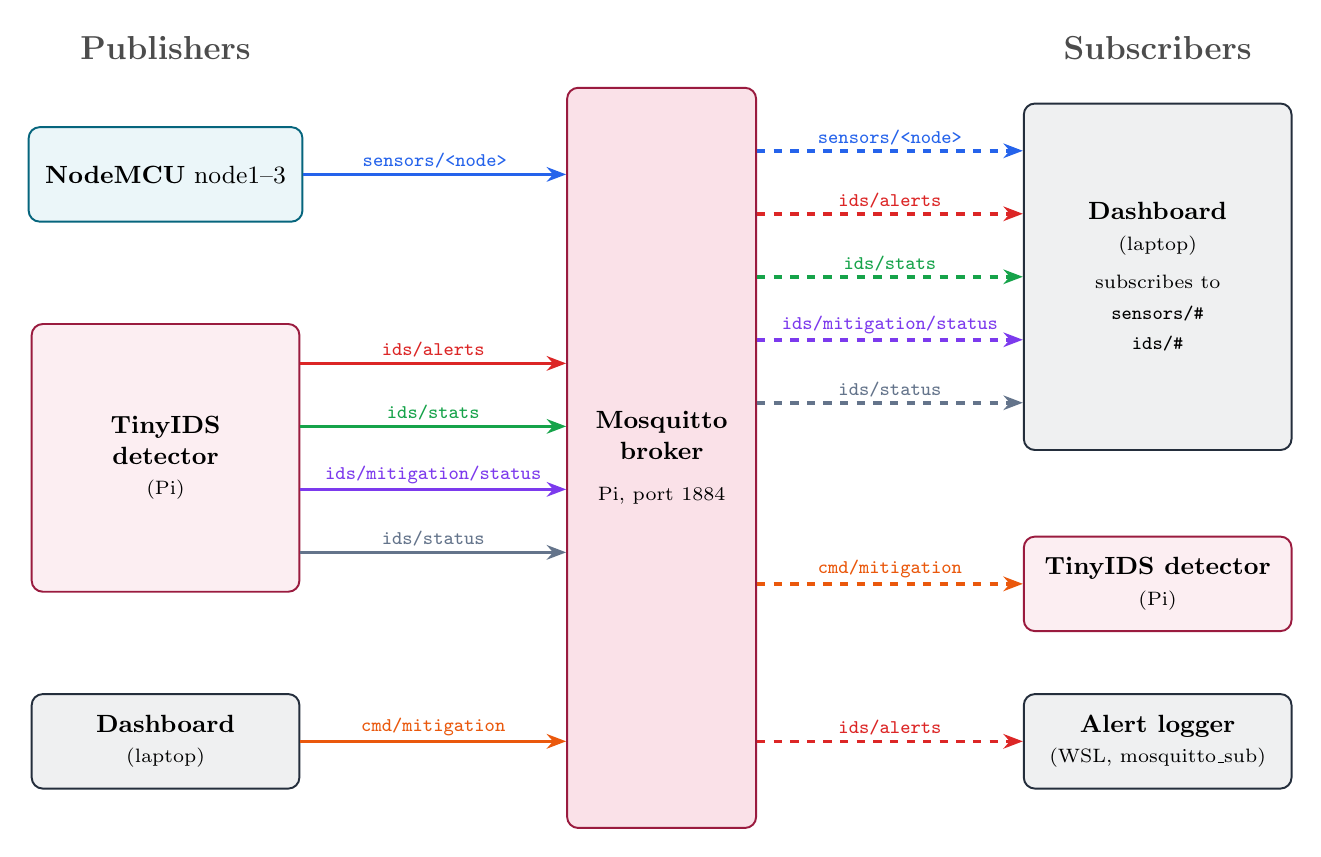
\begin{tikzpicture}[font=\small]

% publishers (left)
\node[font=\bfseries\large, text=gray!60!black] at (1.7,5.2) {Publishers};
\node[box=cNode, minimum width=3.4cm, minimum height=1.2cm] (pN) at (1.7,3.6) {\textbf{NodeMCU} node1--3};
\node[box=cPi, minimum width=3.4cm, minimum height=3.4cm] (pI) at (1.7,0) {\textbf{TinyIDS}\\\textbf{detector}\\{\scriptsize (Pi)}};
\node[box=cLap, minimum width=3.4cm, minimum height=1.2cm] (pD) at (1.7,-3.6) {\textbf{Dashboard}\\{\scriptsize (laptop)}};

% broker
\node[box=cPi, minimum width=2.4cm, minimum height=9.4cm, fill=cPi!14] (B) at (8,0)
  {\textbf{Mosquitto}\\\textbf{broker}\\[4pt]{\scriptsize Pi, port 1884}};

% subscribers (right)
\node[font=\bfseries\large, text=gray!60!black] at (14.3,5.2) {Subscribers};
\node[box=cLap, minimum width=3.4cm, minimum height=4.4cm] (sD) at (14.3,2.3) {\textbf{Dashboard}\\{\scriptsize (laptop)}\\[3pt]{\scriptsize subscribes to}\\{\scriptsize\ttfamily sensors/\#}\\{\scriptsize\ttfamily ids/\#}};
\node[box=cPi, minimum width=3.4cm, minimum height=1.2cm] (sI) at (14.3,-1.6) {\textbf{TinyIDS detector}\\{\scriptsize (Pi)}};
\node[box=cLap, minimum width=3.4cm, minimum height=1.2cm] (sL) at (14.3,-3.6) {\textbf{Alert logger}\\{\scriptsize (WSL, mosquitto\_sub)}};

% incoming (publish), solid
\draw[pub=cSensor] (pN.east) -- node[lbl=cSensor, above] {sensors/<node>} (pN.east -| B.west);
\draw[pub=cAlert]  ($(pI.east)+(0,1.2)$)  -- node[lbl=cAlert, above] {ids/alerts} ($(pI.east -| B.west)+(0,1.2)$);
\draw[pub=cStats]  ($(pI.east)+(0,0.4)$)  -- node[lbl=cStats, above] {ids/stats} ($(pI.east -| B.west)+(0,0.4)$);
\draw[pub=cMit]    ($(pI.east)+(0,-0.4)$) -- node[lbl=cMit, above] {ids/mitigation/status} ($(pI.east -| B.west)+(0,-0.4)$);
\draw[pub=cStatus] ($(pI.east)+(0,-1.2)$) -- node[lbl=cStatus, above] {ids/status} ($(pI.east -| B.west)+(0,-1.2)$);
\draw[pub=cCmd]    (pD.east) -- node[lbl=cCmd, above] {cmd/mitigation} (pD.east -| B.west);

% outgoing (deliver), dashed
\draw[deliver=cSensor] ($(B.east |- sD.east)+(0,1.6)$)  -- node[lbl=cSensor, above] {sensors/<node>} ($(sD.west)+(0,1.6)$);
\draw[deliver=cAlert]  ($(B.east |- sD.east)+(0,0.8)$)  -- node[lbl=cAlert, above] {ids/alerts} ($(sD.west)+(0,0.8)$);
\draw[deliver=cStats]  ($(B.east |- sD.east)+(0,0)$)    -- node[lbl=cStats, above] {ids/stats} ($(sD.west)+(0,0)$);
\draw[deliver=cMit]    ($(B.east |- sD.east)+(0,-0.8)$) -- node[lbl=cMit, above] {ids/mitigation/status} ($(sD.west)+(0,-0.8)$);
\draw[deliver=cStatus] ($(B.east |- sD.east)+(0,-1.6)$) -- node[lbl=cStatus, above] {ids/status} ($(sD.west)+(0,-1.6)$);
\draw[deliver=cCmd]    (B.east |- sI.west) -- node[lbl=cCmd, above] {cmd/mitigation} (sI.west);
\draw[deliver=cAlert]  (B.east |- sL.west) -- node[lbl=cAlert, above] {ids/alerts} (sL.west);

\end{tikzpicture}}
\caption{Every topic in its own colour. \textbf{Solid} = incoming to the broker (publish);
\textbf{dashed} = outgoing from the broker (delivered to a subscriber).}\label{fig:topics}
\end{figure}

\subsection{The topic list}

\tablestart
\begin{longtable}{P{3.9cm}P{2.2cm}P{2.3cm}P{6.0cm}}
\caption*{}\\[-2.5em]
\toprule
Topic & Publisher & Subscribers & When, content and use \\
\midrule
\endhead
\topicdot{cSensor}\; \file{sensors/<node>} \newline {\scriptsize e.g.\ \file{sensors/node1}} & each NodeMCU &
Dashboard (\file{sensors/\#}) & every 2~s: \file{node}, \file{temp\_c}, \file{humidity}, \file{uptime\_s}.
The normal IoT traffic. The dashboard shows each sensor and when it was last seen. \\
\topicdot{cAlert}\; \file{ids/alerts} & TinyIDS detector & Dashboard, alert logger & on every alert: time,
sender (with node name if it is one of our sensors), attack, confidence, the \textbf{top-3 SHAP reasons}, model
time, SHAP time, and whether the model or a rule found it. \\
\topicdot{cStats}\; \file{ids/stats} & TinyIDS detector & Dashboard & every second: packets/s (total and per
sender), windows classified, alerts so far, average model and SHAP time, which IP is which sensor. Feeds the traffic
chart and the counters. \\
\topicdot{cMit}\; \file{ids/mitigation/status} & TinyIDS detector & Dashboard & every second, \emph{retained}: IPS
on/off, the blocked, quarantined and rate-limited IPs with seconds left, the last 10 actions. Feeds the ``Active
Defense'' panel. \\
\topicdot{cStatus}\; \file{ids/status} & TinyIDS detector & Dashboard & once at start, \emph{retained}: start time,
model, number of features, gateway IP. \\
\topicdot{cCmd}\; \file{cmd/mitigation} & Dashboard (buttons) & TinyIDS detector & when a button is pressed:
\file{toggle\_ips} (detect only $\leftrightarrow$ detect + block), \file{flush\_all} (release every blocked IP). The
detector also understands \file{unblock} for one IP. \\
\bottomrule
\end{longtable}

\textbf{Retained} = the broker keeps the last message and gives it to anyone who subscribes later, so a dashboard
opened late still shows the current status at once.

\textbf{The detector also reads \file{sensors/<node>} without subscribing:} it sees the sensors' MQTT packets on the
wire and learns which IP belongs to which node (\file{SensorRegistry}). So no IP address is hard-coded, and an alert
can say ``172.29.x.y (node2)''.

\subsection{Traffic that is not MQTT}

\tablestart
\begin{center}
\begin{tabularx}{\linewidth}{P{3.6cm}P{4.6cm}L}
\toprule
Traffic & From $\rightarrow$ to & Purpose \\
\midrule
\textcolor{cBot}{\textbf{Bot commands}} & bot master (Windows) $\rightarrow$ all NodeMCUs, UDP broadcast port 6667 &
``udp 10'', ``tcp 10'', ``stop''. Like a botnet's command server, but our own hardware only. Never through the
broker \\
\textcolor{cAttack}{\textbf{Bot floods}} & NodeMCUs $\rightarrow$ Pi & UDP to port 5683, or TCP connections to port
1884 (DDoS from 3 senders) \\
\textcolor{cAttack}{\textbf{Laptop attacks}} & WSL $\rightarrow$ Pi & SYN / UDP / ICMP / ACK / PSH-ACK / RST-FIN
floods (hping3), port, OS and vulnerability scans (nmap), MQTT brute force (wrong passwords to port 1884), ARP
spoofing (arpspoof) \\
SSH & laptop $\rightarrow$ Pi & to start and watch the detector; the admin laptop's SSH and open dashboard connection
are not inspected (so the IDS never blocks its own operator) \\
\bottomrule
\end{tabularx}
\end{center}

\subsection{Ports}

\tablestart
\begin{center}
\begin{tabular}{rll}
\toprule
Port & Protocol & Used for \\
\midrule
1884 & TCP (MQTT) & \textbf{our broker}: sensors, detector, dashboard \\
1883 & TCP (MQTT) & the lab's own broker on the Pi (not ours; target of some TCP floods) \\
5683 & UDP & target of the UDP floods (the CoAP port) \\
6667 & UDP & bot master commands (broadcast) and the bots' answers \\
22 & TCP (SSH) & laptop logs in to the Pi \\
\bottomrule
\end{tabular}
\end{center}

% ---------------------------------------------------------------------------------------------------------------
\newpage
\subsection{Inside the detector}

Every packet that arrives at the Pi goes through two paths at the same time: the \textbf{model path} (left) and the
\textbf{rules} (right).

\begin{figure}[H]
\centering
\resizebox{0.92\linewidth}{!}{%
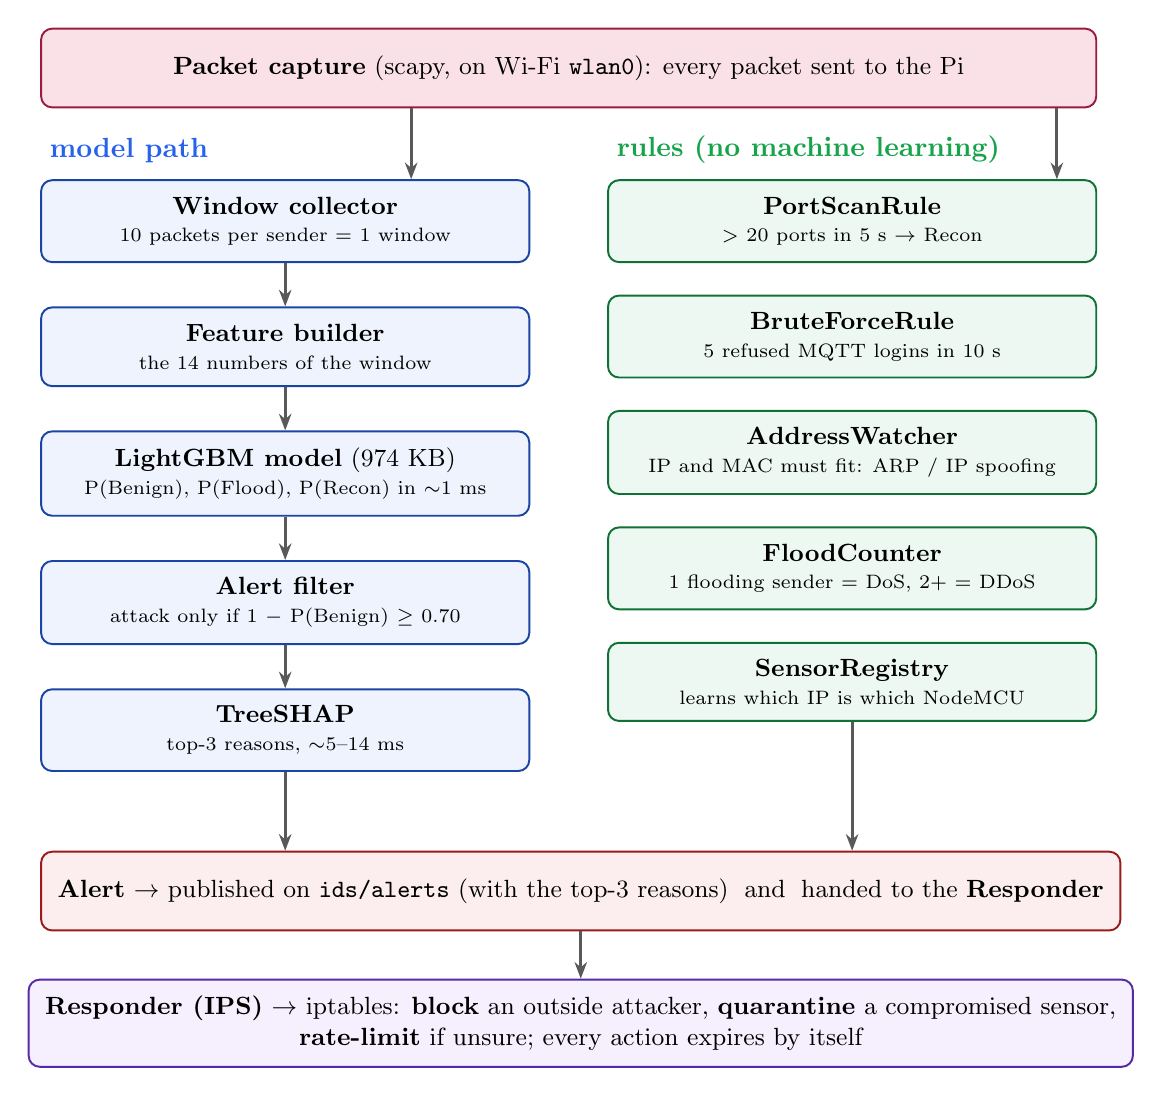
\begin{tikzpicture}[font=\small, node distance=0.55cm]

\node[box=cPi, minimum width=13.4cm, minimum height=1.0cm, fill=cPi!14] (cap)
  {\textbf{Packet capture} (scapy, on Wi-Fi \texttt{wlan0}): every packet sent to the Pi};

\node[box=cSensor, minimum width=6.2cm, minimum height=1.0cm, below=0.9cm of cap.south west, anchor=north west] (win)
  {\textbf{Window collector}\\[-1pt]{\scriptsize 10 packets per sender = 1 window}};
\node[box=cSensor, minimum width=6.2cm, minimum height=1.0cm, below=of win] (feat)
  {\textbf{Feature builder}\\[-1pt]{\scriptsize the 14 numbers of the window}};
\node[box=cSensor, minimum width=6.2cm, minimum height=1.0cm, below=of feat] (lgbm)
  {\textbf{LightGBM model} (974 KB)\\[-1pt]{\scriptsize P(Benign), P(Flood), P(Recon) in $\sim$1 ms}};
\node[box=cSensor, minimum width=6.2cm, minimum height=1.0cm, below=of lgbm] (filt)
  {\textbf{Alert filter}\\[-1pt]{\scriptsize attack only if 1 $-$ P(Benign) $\geq$ 0.70}};
\node[box=cSensor, minimum width=6.2cm, minimum height=1.0cm, below=of filt] (shap)
  {\textbf{TreeSHAP}\\[-1pt]{\scriptsize top-3 reasons, $\sim$5--14 ms}};

\node[box=cStats, minimum width=6.2cm, minimum height=0.85cm, below=0.9cm of cap.south east, anchor=north east] (r1)
  {\textbf{PortScanRule}\\[-1pt]{\scriptsize $>$ 20 ports in 5 s $\rightarrow$ Recon}};
\node[box=cStats, minimum width=6.2cm, minimum height=0.85cm, below=0.4cm of r1] (r2)
  {\textbf{BruteForceRule}\\[-1pt]{\scriptsize 5 refused MQTT logins in 10 s}};
\node[box=cStats, minimum width=6.2cm, minimum height=0.85cm, below=0.4cm of r2] (r3)
  {\textbf{AddressWatcher}\\[-1pt]{\scriptsize IP and MAC must fit: ARP / IP spoofing}};
\node[box=cStats, minimum width=6.2cm, minimum height=0.85cm, below=0.4cm of r3] (r4)
  {\textbf{FloodCounter}\\[-1pt]{\scriptsize 1 flooding sender = DoS, 2+ = DDoS}};
\node[box=cStats, minimum width=6.2cm, minimum height=0.85cm, below=0.4cm of r4] (r5)
  {\textbf{SensorRegistry}\\[-1pt]{\scriptsize learns which IP is which NodeMCU}};

\node[box=cAlert, minimum width=13.4cm, minimum height=1.0cm, below=1.0cm of shap.south west, anchor=north west] (alert)
  {\textbf{Alert} $\rightarrow$ published on \texttt{ids/alerts} (with the top-3 reasons) \;and\; handed to the
  \textbf{Responder}};
\node[box=cMit, minimum width=13.4cm, minimum height=1.0cm, below=0.6cm of alert] (resp)
  {\textbf{Responder (IPS)} $\rightarrow$ iptables: \textbf{block} an outside attacker, \textbf{quarantine} a
  compromised sensor,\\ \textbf{rate-limit} if unsure; every action expires by itself};

\node[font=\bfseries, text=cSensor, anchor=south west] at ($(win.north west)+(0,0.08)$) {model path};
\node[font=\bfseries, text=cStats, anchor=south west] at ($(r1.north west)+(0,0.08)$) {rules (no machine learning)};

\draw[flow] ($(cap.south -| win.north)+(1.6,0)$) -- ($(win.north)+(1.6,0)$);
\draw[flow] ($(cap.south -| r1.north)+(2.6,0)$) -- ($(r1.north)+(2.6,0)$);
\draw[flow] (win) -- (feat); \draw[flow] (feat) -- (lgbm); \draw[flow] (lgbm) -- (filt); \draw[flow] (filt) -- (shap);
\draw[flow] (shap.south) -- (shap.south |- alert.north);
\draw[flow] (r5.south) -- (r5.south |- alert.north);
\draw[flow] (alert) -- (resp);

\end{tikzpicture}}
\caption{The detector on the Pi. Every second it also publishes \texttt{ids/stats} and
\texttt{ids/mitigation/status}, and it listens on \texttt{cmd/mitigation}.}
\end{figure}

\subsection{The life of one attack, step by step}

Example: the 3 NodeMCU bots flood the Pi.

\begin{enumerate}
  \item On the laptop (Windows) \file{python bot.py tcp 10} sends one UDP broadcast ``tcp 10''.
  \item All 3 NodeMCUs switch to bot mode and open TCP connections to the Pi as fast as they can.
  \item On the Pi, every 10 packets from one bot form a window; the 14 features go into the model.
  \item The model says \textbf{Flood} with P(attack) $\geq$ 0.70; TreeSHAP finds the top-3 reasons
        (e.g.\ \file{syn\_flag\_number}, \file{fin\_flag\_number}, \file{rst\_flag\_number}).
  \item The FloodCounter sees 3 senders flooding at once $\rightarrow$ \textbf{DDoS}; the SensorRegistry knows they
        are our own NodeMCUs $\rightarrow$ \textbf{quarantine} (they are compromised).
  \item The Responder adds iptables rules: the kernel drops their packets.
  \item The detector publishes the alert on \file{ids/alerts} and the new state on \file{ids/mitigation/status}.
  \item The broker delivers both to the dashboard: the alert appears with its SHAP bar chart, the 3 nodes appear in
        the quarantine table.
  \item After 10~s the bots stop by themselves; after the quarantine time the rules are removed and the nodes go back
        to normal sensor traffic.
\end{enumerate}

\subsection{The dashboard}

A Streamlit web page on the laptop. It only reads MQTT messages and sends button commands; it never talks to the
detector directly.

\tablestart
\begin{center}
\begin{tabularx}{\linewidth}{P{4.6cm}P{4.2cm}L}
\toprule
Panel & Fed by & Shows \\
\midrule
Counters (top row) & \file{ids/stats}, \file{ids/status} & packets/s, windows, alerts, model and SHAP time \\
Traffic at the gateway & \file{ids/stats} & packets/s over time, per sender \\
Sensors & \file{sensors/<node>} & every NodeMCU, its last reading and when it was last seen \\
Active Defense (IPS) & \file{ids/mitigation/status} & IPS on/off, blocked / quarantined / rate-limited IPs, history;
buttons \textbf{toggle IPS} and \textbf{Flush Bans} publish \file{cmd/mitigation} \\
Alerts & \file{ids/alerts} & table of alerts, coloured by attack type (button: clear alerts, only on the page) \\
Why? (SHAP) & \file{ids/alerts} & bar chart of the top-3 SHAP features of the latest alert of each type \\
\bottomrule
\end{tabularx}
\end{center}

% ---------------------------------------------------------------------------------------------------------------
\section{The data}

\subsection{The dataset: CICIoT2023}

A public dataset recorded in a lab with 105 IoT devices. Our copy has \textbf{7.85 million rows}, 46 features and
34 labels (benign + 33 attacks). The authors already split it into three files:

\begin{center}
\begin{tabular}{lrr}
\toprule
File & Rows & Share \\
\midrule
\file{train.csv} & 5,491,971 & 70\% \\
\file{validation.csv} & 1,176,851 & 15\% \\
\file{test.csv} & 1,176,851 & 15\% \\
\bottomrule
\end{tabular}
\end{center}

Only \textbf{2.36\%} of the rows are benign; DDoS + DoS floods are 90\% of everything.

\subsection{The 13 labels we kept}

\begin{center}
\begin{tabularx}{\linewidth}{P{2.6cm}L}
\toprule
Our class & Dataset labels \\
\midrule
\textbf{Benign} & \file{BenignTraffic} \\
\textbf{Flood} (9) & \file{DDoS-SYN\_Flood}, \file{DDoS-UDP\_Flood}, \file{DDoS-ICMP\_Flood}, \file{DDoS-TCP\_Flood},
\file{DDoS-PSHACK\_Flood}, \file{DDoS-RSTFINFlood}, \file{DoS-SYN\_Flood}, \file{DoS-UDP\_Flood},
\file{DoS-TCP\_Flood} \\
\textbf{Recon} (3) & \file{Recon-PortScan}, \file{Recon-OSScan}, \file{VulnerabilityScan} \\
\bottomrule
\end{tabularx}
\end{center}

\subsection{The 21 labels we dropped, and why}

All 21 by name. The last column is measured on the dataset's test rows: how often the model still calls them an
attack, although it never trained on them.

\tablestart
\begin{longtable}{P{11.5cm}r}
\toprule
Dropped label (grouped, with the reason) & Still detected \\
\midrule
\endhead
\multicolumn{2}{l}{\textit{Web attacks (6): need a web server; the Pi has none, so they cannot be tested. 0.05\% of rows}} \\
\file{SqlInjection} & 4.7\% \\
\file{XSS} & 0\% \\
\file{CommandInjection} & 0\% \\
\file{Backdoor\_Malware} & 2.2\% \\
\file{BrowserHijacking} & 2.2\% \\
\file{Uploading\_Attack} & 0\% \\
\midrule
\multicolumn{2}{l}{\textit{Mirai (3): needs real Mirai malware; our NodeMCU bots already make real DDoS floods}} \\
\file{Mirai-greeth\_flood} & 99.4\% \\
\file{Mirai-greip\_flood} & 99.1\% \\
\file{Mirai-udpplain} & 99.4\% \\
\midrule
\multicolumn{2}{l}{\textit{Spoofing (2): rows have no IP / MAC columns, so they cannot show it; a rule handles it}} \\
\file{MITM-ArpSpoofing} & 9.3\% \\
\file{DNS\_Spoofing} & 14.8\% \\
\midrule
\multicolumn{2}{l}{\textit{Brute force (1): not MQTT, only 1,541 rows; a rule counts refused MQTT logins}} \\
\file{DictionaryBruteForce} & 2.5\% \\
\midrule
\multicolumn{2}{l}{\textit{HTTP floods (3): need a web server}} \\
\file{DoS-HTTP\_Flood} & 61.0\% \\
\file{DDoS-HTTP\_Flood} & 40.1\% \\
\file{DDoS-SlowLoris} & 19.9\% \\
\midrule
\multicolumn{2}{l}{\textit{Other floods (4): never recorded or tested on our testbed; kept out to stay simple}} \\
\file{DDoS-SynonymousIP\_Flood} & 99.9\% \\
\file{DDoS-ICMP\_Fragmentation} & 97.7\% \\
\file{DDoS-UDP\_Fragmentation} & 66.2\% \\
\file{DDoS-ACK\_Fragmentation} & 43.8\% \\
\midrule
\multicolumn{2}{l}{\textit{Tiny scans (2): fewer than 10 packets reach the Pi, so never a full window}} \\
\file{Recon-PingSweep} & 11.3\% \\
\file{Recon-HostDiscovery} & 50.6\% \\
\bottomrule
\end{longtable}

\textbf{Total: 34 labels = 13 kept + 21 dropped.} Floods that look like our floods (Mirai, SynonymousIP, ICMP
fragmentation) are still caught at 98--99.9\%. Web attacks, brute force and spoofing are not (0--15\%): they look
like normal traffic in these features, which is expected; rules cover spoofing and brute force.

\subsection{Why all floods are ONE class}

\begin{enumerate}
  \item \textbf{The response is the same:} whatever the flood type, the Pi blocks the sender.
  \item \textbf{The type is still visible:} the SHAP reasons name it (\file{syn\_flag\_number} = SYN flood,
        \file{UDP} = UDP flood, \file{ICMP} = ping flood); see Section~\ref{sec:attackfeatures}.
  \item \textbf{DoS vs DDoS cannot be learned from one row:} the only difference is how many senders, and rows have
        no addresses. A rule counts the senders instead.
  \item \textbf{Fewer classes = smaller, more reliable model:} 3 classes fit in under 1~MB; the old 8-class model
        reached only about 0.70 macro-F1, mostly by confusing look-alike attacks.
\end{enumerate}

The same for scans: port, OS and vulnerability scan become one class \textbf{Recon}.

\subsection{Our own recordings}

We recorded \textbf{51,843 rows} ourselves, with the same feature code the Pi uses live: 25 recordings in a Docker
testbed and in the real lab (NodeMCU sensors sending MQTT, floods from a laptop and from NodeMCU bots, nmap scans).
They are added to the dataset rows. Before we added our benign rows, the real NodeMCUs caused false ``Recon''
alarms; after, none.

% ---------------------------------------------------------------------------------------------------------------
\section{The features}

\subsection{The 14 features we use, and why only these}

Every dataset row has 46 features. We use only the 14 that our Pi computes \textbf{exactly the same way} as the
dataset (we measured this by recording our own floods and comparing them with the dataset's floods). If the model
learned from a feature the Pi computes differently, it would score well in training and fail live.

\tablestart
\begin{center}
\begin{tabularx}{\linewidth}{rP{4.2cm}L}
\toprule
\# & Feature & Meaning (per window of 10 packets) \\
\midrule
1 & \file{Protocol Type} & most common protocol (6 = TCP, 17 = UDP, 1 = ICMP) \\
2 & \file{TCP} & share of TCP packets \\
3 & \file{UDP} & share of UDP packets \\
4 & \file{ICMP} & share of ICMP (ping) packets \\
5 & \file{syn\_flag\_number} & share of packets with the SYN flag \\
6 & \file{ack\_flag\_number} & share with the ACK flag \\
7 & \file{psh\_flag\_number} & share with the PSH flag \\
8 & \file{rst\_flag\_number} & share with the RST flag \\
9 & \file{fin\_flag\_number} & share with the FIN flag \\
10 & \file{Min} & smallest packet size \\
11 & \file{Max} & largest packet size \\
12 & \file{AVG} & average packet size \\
13 & \file{Std} & how much the packet sizes vary \\
14 & \file{Tot size} & average packet length \\
\bottomrule
\end{tabularx}
\end{center}

\subsection{Which features decide each attack}\label{sec:attackfeatures}

One model, one decision per window, always using all 14 features. These are the features that mattered most for
each attack (SHAP top-3, measured live on the real Pi, 17 November). This is how an alert shows the
\emph{kind} of flood although the class is just ``Flood''.

\tablestart
\begin{center}
\begin{tabularx}{\linewidth}{P{5.2cm}L}
\toprule
Attack & Main features (SHAP top-3) \\
\midrule
UDP flood & \file{Protocol Type}, \file{UDP}, \file{Min} \\
ICMP (ping) flood & \file{ICMP}, \file{Min} \\
SYN flood & \file{syn\_flag\_number}, \file{Min}, \file{Std} \\
ACK flood & \file{Min}, \file{Max}, \file{Std} \\
PSH-ACK flood & \file{psh\_flag\_number}, \file{Min}, \file{Max} \\
RST-FIN flood & \file{fin\_flag\_number}, \file{rst\_flag\_number}, \file{Min} \\
Bot TCP flood (DDoS, NodeMCU bots) & \file{syn\_flag\_number}, \file{fin\_flag\_number}, \file{rst\_flag\_number} \\
Port / version scan (Recon) & \file{AVG}, \file{Tot size}, \file{Max}, \file{Protocol Type} \\
Normal NodeMCU traffic & bigger packets (\file{Tot size}, \file{AVG}), PSH / ACK flags \\
\bottomrule
\end{tabularx}
\end{center}

\subsection{The 32 features we dropped}

\tablestart
\begin{center}
\begin{tabularx}{\linewidth}{P{4.6cm}Lr}
\toprule
Reason & Features & Count \\
\midrule
Computed differently live than in the dataset & \file{flow\_duration}, \file{Header\_Length}, \file{Rate},
\file{Srate}, \file{Drate}, \file{Duration}, \file{LLC} & 7 \\
Shortcuts that give away the answer & \file{IAT} (capture time), \file{Number}, \file{Weight} (window size) & 3 \\
Count and statistics features we do not compute live & \file{ack\_count}, \file{syn\_count}, \file{fin\_count},
\file{urg\_count}, \file{rst\_count}, \file{Tot sum}, \file{Magnitue}, \file{Radius}, \file{Covariance},
\file{Variance} & 10 \\
Always 0 (or always 1) for our attacks & \file{HTTP}, \file{HTTPS}, \file{DNS}, \file{Telnet}, \file{SMTP},
\file{SSH}, \file{IRC}, \file{DHCP}, \file{ARP}, \file{IPv}, \file{ece\_flag\_number}, \file{cwr\_flag\_number} & 12 \\
\midrule
\textbf{Total dropped} & & \textbf{32} \\
\bottomrule
\end{tabularx}
\end{center}

\keybox{\textbf{In one line:} the model only looks at packet sizes, TCP flags and protocol: 14 numbers per 10
packets, computed exactly the same way on the Pi as in the dataset, so what it learned in training also works live.}

% ---------------------------------------------------------------------------------------------------------------
\section{Train, validation and test}

\subsection{What each one is for}

Think of a student preparing for an exam:

\tablestart
\begin{center}
\begin{tabularx}{\linewidth}{P{2.3cm}P{3.3cm}L}
\toprule
Set & Like & What it does for our model \\
\midrule
\textbf{Train} & the textbook & the model \textbf{learns} from these rows: it sees the 14 numbers and the right
answer and builds its trees \\
\textbf{Validation} & practice tests while studying & not learned from. After every new tree the score on them is
checked; when it stops improving, training stops (prevents memorising) \\
\textbf{Test} & the final exam & \textbf{never seen} during training; used once at the end for the real score \\
\bottomrule
\end{tabularx}
\end{center}

Testing on rows the model trained on is like giving the student the exam questions in advance: a great score that
means nothing.

\subsection{How the dataset rows were used}

We did not split anything ourselves: we used the authors' three files, removed the 21 dropped labels from
\emph{all three}, and took a random 20\% (the same 20\% of every attack type) from two of them.

\tablestart
\begin{center}
\begin{tabular}{lrlr}
\toprule
File & After removing & Then & Used as \\
\midrule
\file{train.csv} & 4.55 M & 20\% $\rightarrow$ \textbf{909,368} & training \\
\file{validation.csv} & 974 K & 20\% $\rightarrow$ \textbf{194,837} & validation \\
\file{test.csv} & 973,829 & \textbf{all}, no cut & test \\
\bottomrule
\end{tabular}
\end{center}

Why only 20\%? 900,000 rows is already plenty for this model; more rows make training slower, not better
(early stopping decides when it has learned enough).

\subsection{How our own rows were used: split by time}\label{sec:timesplit}

Each of our recordings is a list of windows in time order. Neighbouring windows (a fraction of a second apart, same
attack) have almost the same numbers. So we split by \textbf{time}, not by picking rows at random: in every
recording, separately for its normal rows and its attack rows,

\begin{itemize}
  \item the \textbf{first 70\%} of the rows $\rightarrow$ train,
  \item the \textbf{next 15\%} $\rightarrow$ validation,
  \item the \textbf{last 15\%} $\rightarrow$ test.
\end{itemize}

Example with one recording of 10 windows: train = 1--7, validation = 8, test = 9--10. Train and test meet at only
one point in time, so the test rows are close to new traffic. (Picking rows at random would put window 6 in the
test and windows 5 and 7 in training: the model would practically have seen it already.) The split is made per
class because nmap scans finish early in a recording: the last 15\% of a whole scan recording contains no scan rows.

\tablestart
\begin{center}
\begin{tabular}{lrrrr}
\toprule
Our rows & Total & Benign (NodeMCU) & Flood & Recon \\
\midrule
$\rightarrow$ train (first 70\%) & 36,279 & 2,621 & 33,489 & 169 \\
$\rightarrow$ validation (next 15\%) & 7,775 & 562 & 7,178 & 35 \\
$\rightarrow$ \textbf{test (last 15\%)} & \textbf{7,789} & \textbf{564} & 7,185 & 40 \\
\bottomrule
\end{tabular}
\end{center}

The results on our own traffic (Section~\ref{sec:ourresults}) are measured this way. The deployed model on the Pi
was trained with the same recipe on all the same dataset rows, with 70\% of our rows picked at random for training
(36,255 rows).

\textbf{Training total of the deployed model:} 945,623 rows (909,368 dataset + 36,255 ours): 911,821 Flood, 28,507
Benign, 5,295 Recon.

% ---------------------------------------------------------------------------------------------------------------
\Needspace{16\baselineskip}
\section{Class imbalance and class weights}\label{sec:weights}

\subsection{The problem}

The training rows are very unequal:

\tablestart
\begin{center}
\begin{tabular}{lrr}
\toprule
Class & Training rows & Share \\
\midrule
Flood & 911,821 & 96.4\% \\
Benign & 28,507 & 3.0\% \\
Recon & 5,295 & 0.6\% \\
\bottomrule
\end{tabular}
\end{center}

A lazy model could answer ``Flood'' for every window and still be \textbf{96\% right}, while never recognising a
normal sensor or a scan. While training, the model tries to make as few mistakes as possible in total; with 172
Flood rows for every Recon row, getting Recon wrong costs it almost nothing. This is called \textbf{class
imbalance}.

\subsection{The fix we used: class weights}

Every training row gets a \textbf{weight}: how much a mistake on that row counts. Rows of rare classes count more.

\textbf{Formula} (per class): weight = $\sqrt{\dfrac{\text{all rows}}{3 \times \text{rows of this class}}}$, then
all weights are scaled so that the average row weight is 1.

\tablestart
\begin{center}
\begin{tabular}{lrrr}
\toprule
Class & Share of rows & Weight per row & Compared with one Flood row \\
\midrule
Flood & 96.4\% & 0.83 & 1$\times$ \\
Benign & 3.0\% & 4.68 & \textbf{5.7$\times$} \\
Recon & 0.6\% & 10.86 & \textbf{13$\times$} \\
\bottomrule
\end{tabular}
\end{center}

So one Recon mistake hurts the model as much as 13 Flood mistakes, and one Benign mistake as much as 6.

\subsection{Why the square root, not the full inverse}

The full inverse ($\frac{\text{all rows}}{3 \times \text{rows of this class}}$, no square root) would make every
class count exactly the same in total: one Recon row would count \textbf{172$\times$} a Flood row. That pushes the
model hard towards ``Recon'' and risks normal traffic being called a scan (false alarms). The square root is the
middle way: rare classes matter much more, without pushing that hard. (We did not train a full-inverse version to
compare; this is the usual reasoning, not a measurement.)

\subsection{What we did NOT use}

\begin{itemize}
  \item \textbf{Oversampling / SMOTE} (copying rare rows or inventing new ones): weights do the same job without
        making the training data bigger or adding invented rows.
  \item \textbf{Undersampling} (throwing away Flood rows): would waste real data.
\end{itemize}

\subsection{The second safety net: the 0.70 threshold}

The model gives three probabilities. A window is called an attack only if P(attack) = 1 $-$ P(Benign) is at least
\textbf{0.70}, not just more than 0.5. So the model must be quite sure before it raises an alarm. Weights help rare
classes get noticed; the threshold keeps false alarms on our sensors low.

\subsection{Did it work?}

Partly. Benign is recognised 99\% of the time and our own sensors get no false alarms. \textbf{Recon is still the
weakest class}: 29\% of the dataset's scan rows and 78\% of our own scan rows are caught
(Section~\ref{sec:results}). Many of the dataset's scan rows simply look like normal traffic in these 14 features,
and no weighting can fix that.

% ---------------------------------------------------------------------------------------------------------------
\section{How the model was trained}

The code is \file{retrain/train\_model14.ipynb} (step by step, with explanations); it rebuilds exactly the model
that runs on the Pi.

\textbf{LightGBM} = many small decision trees; each new tree corrects the mistakes of the previous ones
(gradient boosting).

\tablestart
\begin{center}
\begin{tabularx}{\linewidth}{P{3.4cm}P{4.6cm}L}
\toprule
Setting & Value & Why \\
\midrule
Tree size & 15 leaves, 63 value bins & small trees: small file, fast on the Pi \\
Number of trees & up to 300 per class; early stopping after 20 rounds without improvement $\rightarrow$
\textbf{189} & stop before it overfits \\
Class weights & Benign 4.68, Flood 0.83, Recon 10.86 & class imbalance (Section~\ref{sec:weights}) \\
Randomness & 80\% rows and 80\% features per tree, fixed seed & less overfitting; same result every run \\
Decision rule & P(attack) = 1 $-$ P(Benign); below \textbf{0.70} $\rightarrow$ Benign & fewer false alarms \\
File size & \textbf{974 KB} & target: under 1 MB \\
\bottomrule
\end{tabularx}
\end{center}

\textbf{Pruning:} yes, in the tree sense: small trees, early stopping, and a size cap (trees are cut from the end if
the file reaches 1~MB; not needed here).

\textbf{Quantization (INT8): no, not for this model.} A tree model stores split thresholds, not large weight
matrices, and it is already under 1~MB and about 1~ms per window on the Pi. ONNX / INT8 versions of other models
(pruned LightGBM and Random Forest, MLP, 1D-CNN) were built for the model comparison; the deployed detector keeps
LightGBM's own format because the SHAP explanations need it.

% ---------------------------------------------------------------------------------------------------------------
\section{How to read the results}

\begin{itemize}
  \item \textbf{Precision} (per class): when the model says ``Flood'', how often it really is a flood.
  \item \textbf{Recall} or \textbf{detection rate}: of all real floods, how many the model caught.
  \item \textbf{F1}: precision and recall combined into one number; 1.0 is perfect.
  \item \textbf{Macro-F1}: the plain average of the classes' F1. Every class counts the same, so a weak small class
        pulls it down. Example: Benign 0.90, Flood 0.998, Recon 0.38 $\rightarrow$ macro-F1 = 0.76.
  \item \textbf{Weighted-F1}: the same average, weighted by the number of rows (here 0.992: the big Flood class hides
        Recon). \textbf{Micro-F1} counts all rows together and equals accuracy (0.993).
  \item \textbf{Confusion matrix}: rows = the truth, columns = what the model said. The diagonal is correct.
  \item \textbf{False-positive rate}: share of normal rows wrongly flagged (false alarms).
  \item \textbf{ROC-AUC}: how well the attack probability separates attack from normal over all thresholds
        (1.0 = perfect, 0.5 = coin flip).
\end{itemize}

% ---------------------------------------------------------------------------------------------------------------
\section{Results}\label{sec:results}

\subsection{On the dataset's test rows (973,829 rows, never used in training)}

\tablestart
\begin{center}
\begin{tabular}{lrrrr}
\toprule
Class & Rows & Precision & Recall & F1 \\
\midrule
Benign & 27,709 & 0.827 & 0.990 & 0.901 \\
Flood & 940,692 & 1.000 & 0.997 & 0.998 \\
Recon & 5,428 & 0.560 & 0.287 & 0.380 \\
\bottomrule
\end{tabular}
\end{center}

\textbf{Attack or not (the main IDS question):} F1 \textbf{0.997}, detection rate \textbf{99.4\%}, false alarms
\textbf{0.97\%}, ROC-AUC \textbf{0.999}. Every flood type is caught at 99.1--99.9\%.

\textbf{Weak spot:} Recon (scans). Most of the dataset's scan rows look like normal traffic with these 14 features,
so only 29\% are caught. In the live lab our nmap scans were caught (and a port-scan rule also fires).

\begin{figure}[H]
\centering
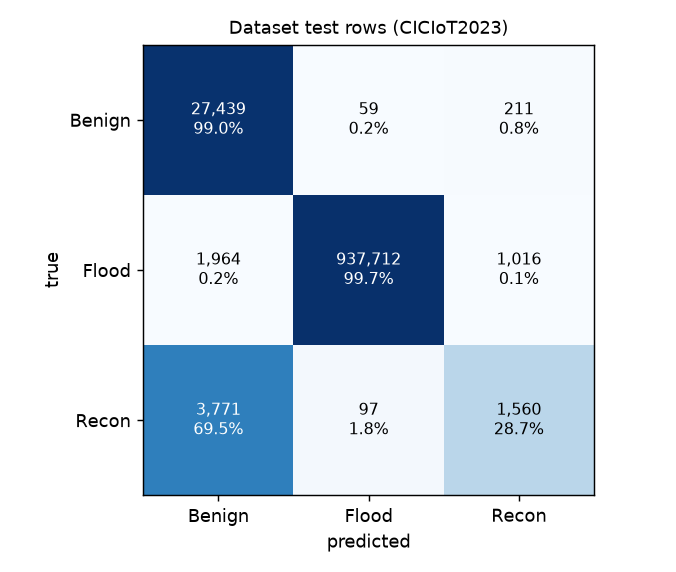
\includegraphics[width=0.62\linewidth]{images/cm_dataset_test.png}
\caption{Confusion matrix on the dataset's test rows.}
\end{figure}

\subsection{On our own traffic (last 15\% of every recording, 7,789 rows)}\label{sec:ourresults}

Split by time as in Section~\ref{sec:timesplit}.

\tablestart
\begin{center}
\begin{tabular}{lrrrr}
\toprule
Class & Rows & Precision & Recall & F1 \\
\midrule
Benign & 564 & 0.995 & 1.000 & 0.997 \\
Flood & 7,185 & 0.999 & 0.999 & 0.999 \\
Recon & 40 & 0.912 & 0.775 & 0.838 \\
\bottomrule
\end{tabular}
\end{center}

Macro-F1 \textbf{0.945}. Our NodeMCU benign traffic: \textbf{564 of 564 correct, 0 false alarms}. Floods: 7,181 of
7,185 caught. Scans: 31 of 40 caught; 7 of the 9 missed scan rows were called ``Flood'' (wrong name, but still
blocked): 7 from the real-lab scan recording, 1 from the OS scan, 1 from the vulnerability scan.

\begin{figure}[H]
\centering
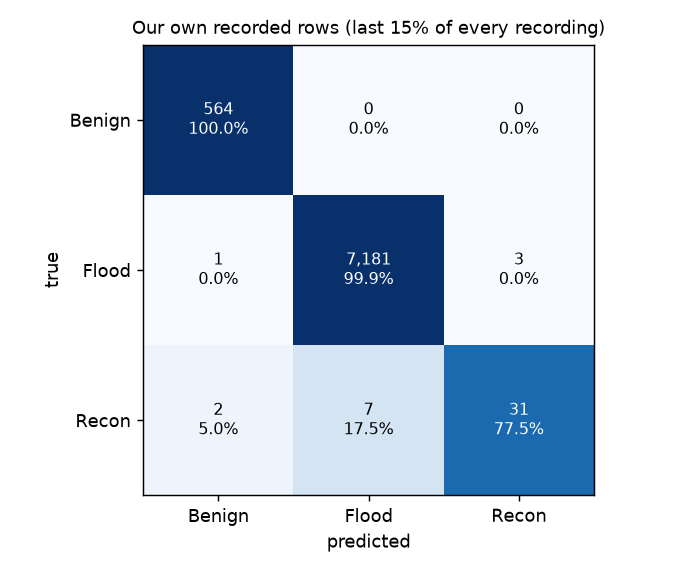
\includegraphics[width=0.62\linewidth]{images/cm_our_rows.png}
\caption{Confusion matrix on our own traffic (last 15\% of every recording).}
\end{figure}

\begin{figure}[H]
\centering
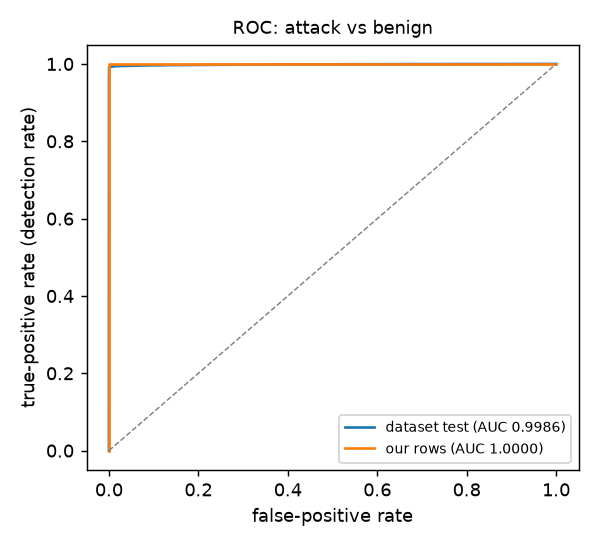
\includegraphics[width=0.56\linewidth]{images/roc_attack_vs_benign.png}
\caption{ROC curve: attack vs benign, on both test sets.}
\end{figure}

\subsection{Live on the real Raspberry Pi (17 November)}

Fresh attacks and fresh NodeMCU traffic, recorded after training, never seen in any form:
\textbf{every attack detected and blocked, zero false alarms on the 3 NodeMCUs.}

\tablestart
\begin{center}
\begin{tabular}{lll}
\toprule
Measure & On the Pi & Target \\
\midrule
Model file size & 974 KB & under 1 MB \\
Time per decision & about 0.7--1.4 ms & under 5 ms \\
SHAP reasons per alert & about 5--14 ms & under 50 ms \\
RAM of the whole detector & 77--78 MB & under 100 MB \\
\bottomrule
\end{tabular}
\end{center}

\subsection{Which features matter most overall}

\begin{figure}[H]
\centering
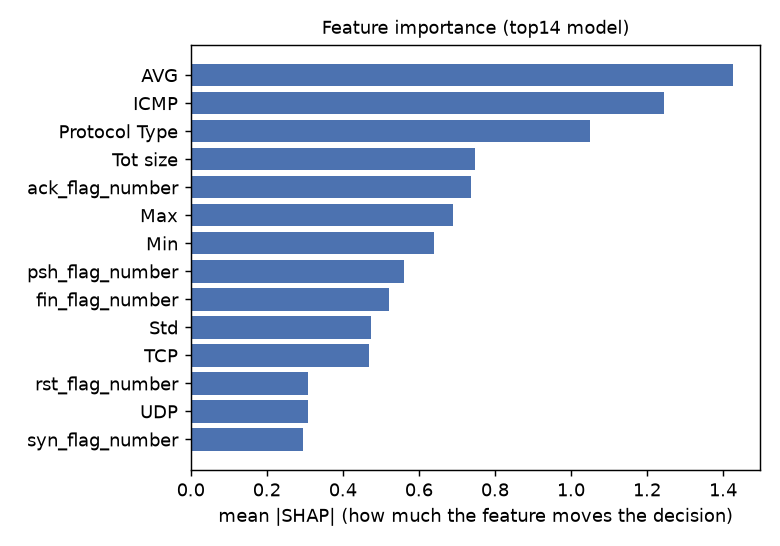
\includegraphics[width=0.68\linewidth]{images/feature_importance.png}
\caption{Feature importance of the deployed model (mean |SHAP| and gain).}
\end{figure}

Packet size (\file{AVG}, \file{Tot size}, \file{Max}, \file{Min}) and protocol decide most cases; the TCP flags
separate the flood types (Section~\ref{sec:attackfeatures}).

% ---------------------------------------------------------------------------------------------------------------
\section{Where everything is}

All paths are relative to the \file{retrain/} folder.

\tablestart
\begin{center}
\begin{tabularx}{\linewidth}{P{4.8cm}L}
\toprule
What & Where \\
\midrule
Training code & \file{train\_model14.ipynb} (same as \file{training/train.py}) \\
Exact rows the deployed model was trained and tested on & \file{evaluation\_matrices/dataset/} (4 csv files + README) \\
The model on the Pi & \file{pi/models/top14/} (copy in \file{evaluation\_matrices/model/}) \\
Detector, broker config, recorder & \file{pi/} (\file{run\_tinyids.py}, \file{tinyids/}, \file{broker/}, \file{record.py}) \\
Dashboard, bot master, attack tools & \file{laptop/} (\file{dashboard.py}, \file{bot.py}, \file{launch.py}, \file{attack\_all.sh}) \\
NodeMCU firmware & \file{laptop/nodemcu\_bot/}, \file{nodemcu\_sensor/}, \file{nodemcu\_sensor\_plain/} \\
Full results tables & \file{evaluation\_matrices/REPORT.md}, pictures in \file{images/} \\
Evaluation code & \file{evaluation\_matrices/evaluate.py} \\
Questions and answers & \file{evaluation\_matrices/data\_and\_model\_questions.md} \\
Our raw recordings & \file{training/data/} \\
Live lab results & \file{RESULTS.md} \\
\bottomrule
\end{tabularx}
\end{center}

\end{document}
